\chapter{System Design}
As described in previous sections, my demonstration system consists of two main parts, namely the on card integrated  communication stack and android application. Figure~\ref{fig:whole-structure} illustrates the request and corresponding response message exchange  process that occurs in the demonstration system.

\begin{figure}[!htbp]
	\centering
	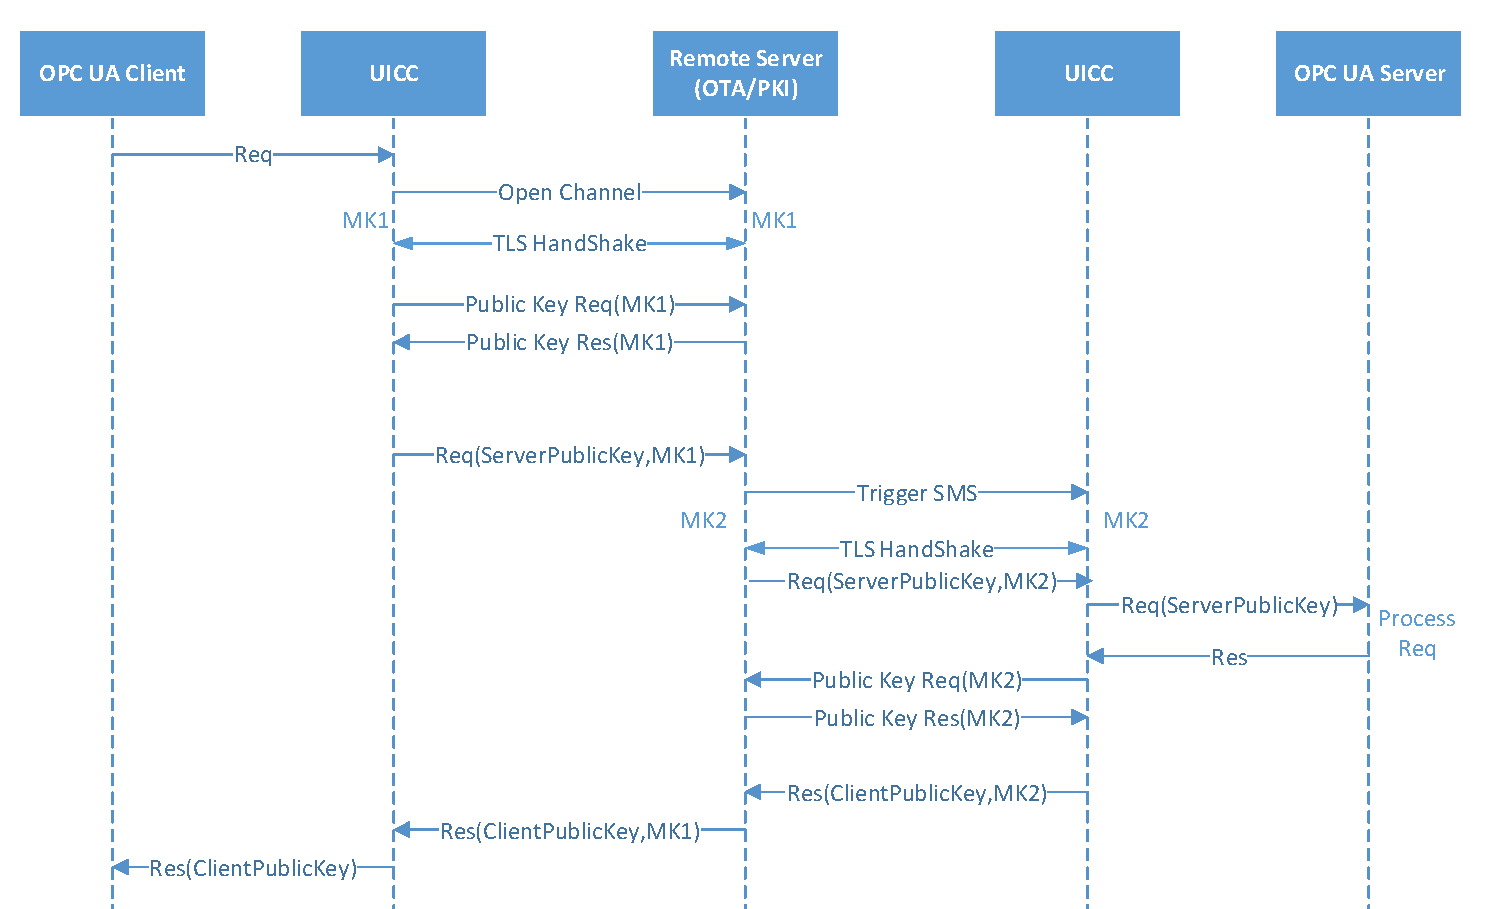
\includegraphics[width=1\textwidth]{whole-structure}
		\caption{Message Exchange}
	\label{fig:whole-structure}
\end{figure}

\section{UICC Applet}

\subsection{Classes}
My UICC applet is developed on Morpho \emph{SC5-01OS07} LTE SAT product.
Communication stack includes following classes:
 \begin{itemize}
  \item  \emph{CommunicationStack}, which is the main class of my applet, that implements \emph{install}, \emph{select}, \emph{deselect} as well as \emph{process} methods provided by \emph{javacard.framework.Applet}. In order to process remote APDU, this applet is also design as UICC system applet, that extends interface \emph{com.orga.javacard.componentinterfaces.JCISIMApplication}
  \item  \emph{AdminTrigger}, which implements Globalplatform  and toolkitframework interfaces and offers functions for proactive and passive communication session creation with OTA server, cipher suit negotiation and mutual authentication.
\end{itemize}

\begin{figure}[!htbp]
	\centering
	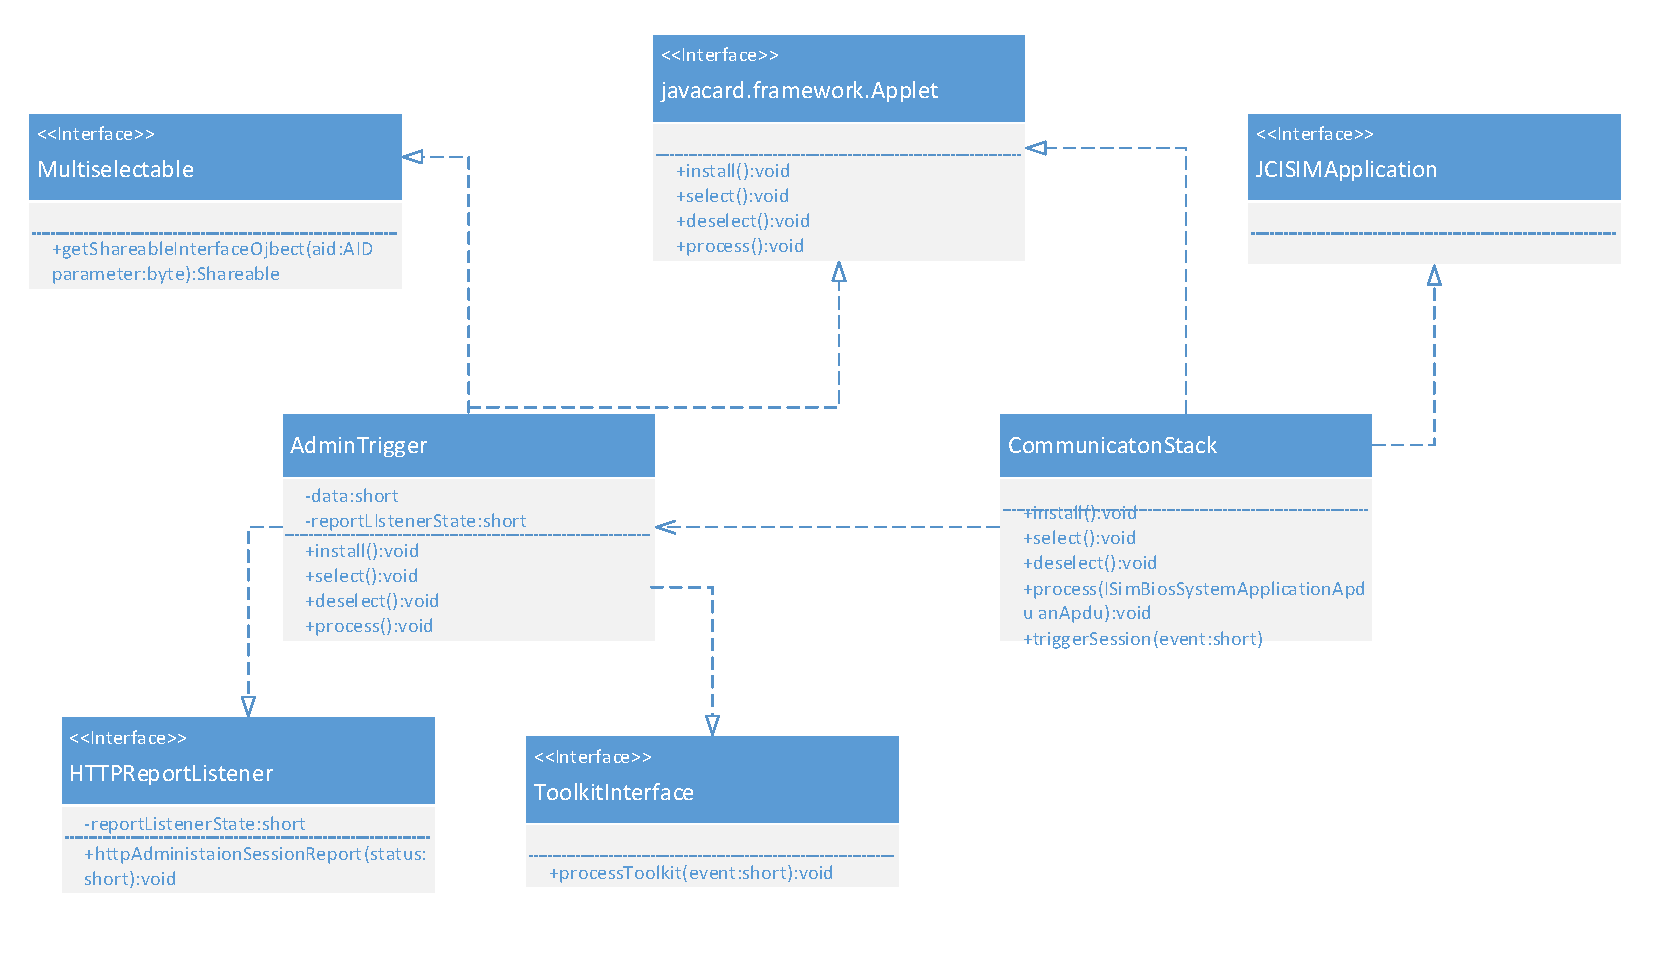
\includegraphics[width=1.0\textwidth]{class}
		\caption{Class Diagram}
	\label{fig:class}
\end{figure}

\subsection {Communication Flow}

The components involved in this scenario are:
 \begin{itemize}
  \item CommunicationStack applet and associated Security Domain from Globalplatform (APSD  for short)
  \item OTA server which is also known as Remote Administration Server (RAS for short)
\end{itemize}

The communication between CommunicationStack and Remote Administration Server involves following  steps:

 \begin{itemize}
  \item Open Communication Channel and Create Communication Session
  \item Secure Message Exchange
  \item Close Communication Session
\end{itemize}
\subsubsection{Communication Session Creation and Message Exchange}
This process could be either initiated by Remote Administration Server by sending target applet a trigger SMS or be sponsored by applet itself. In both cases, applet sends the first \emph{OpenChannel Request} message. During the PSK TLS Handshake phase, APSD and remote server will agree on to be used cipher suit and authenticate each other. After a successful PSK TLS Handshake, CommunicationStack and remote OTA server will be able to exchange HTTP message,that encapsulates APDU strings as body, with HTTP header that is in compliance with GlobalPlatform standards.


\begin{figure}[!htbp]

	\centering
	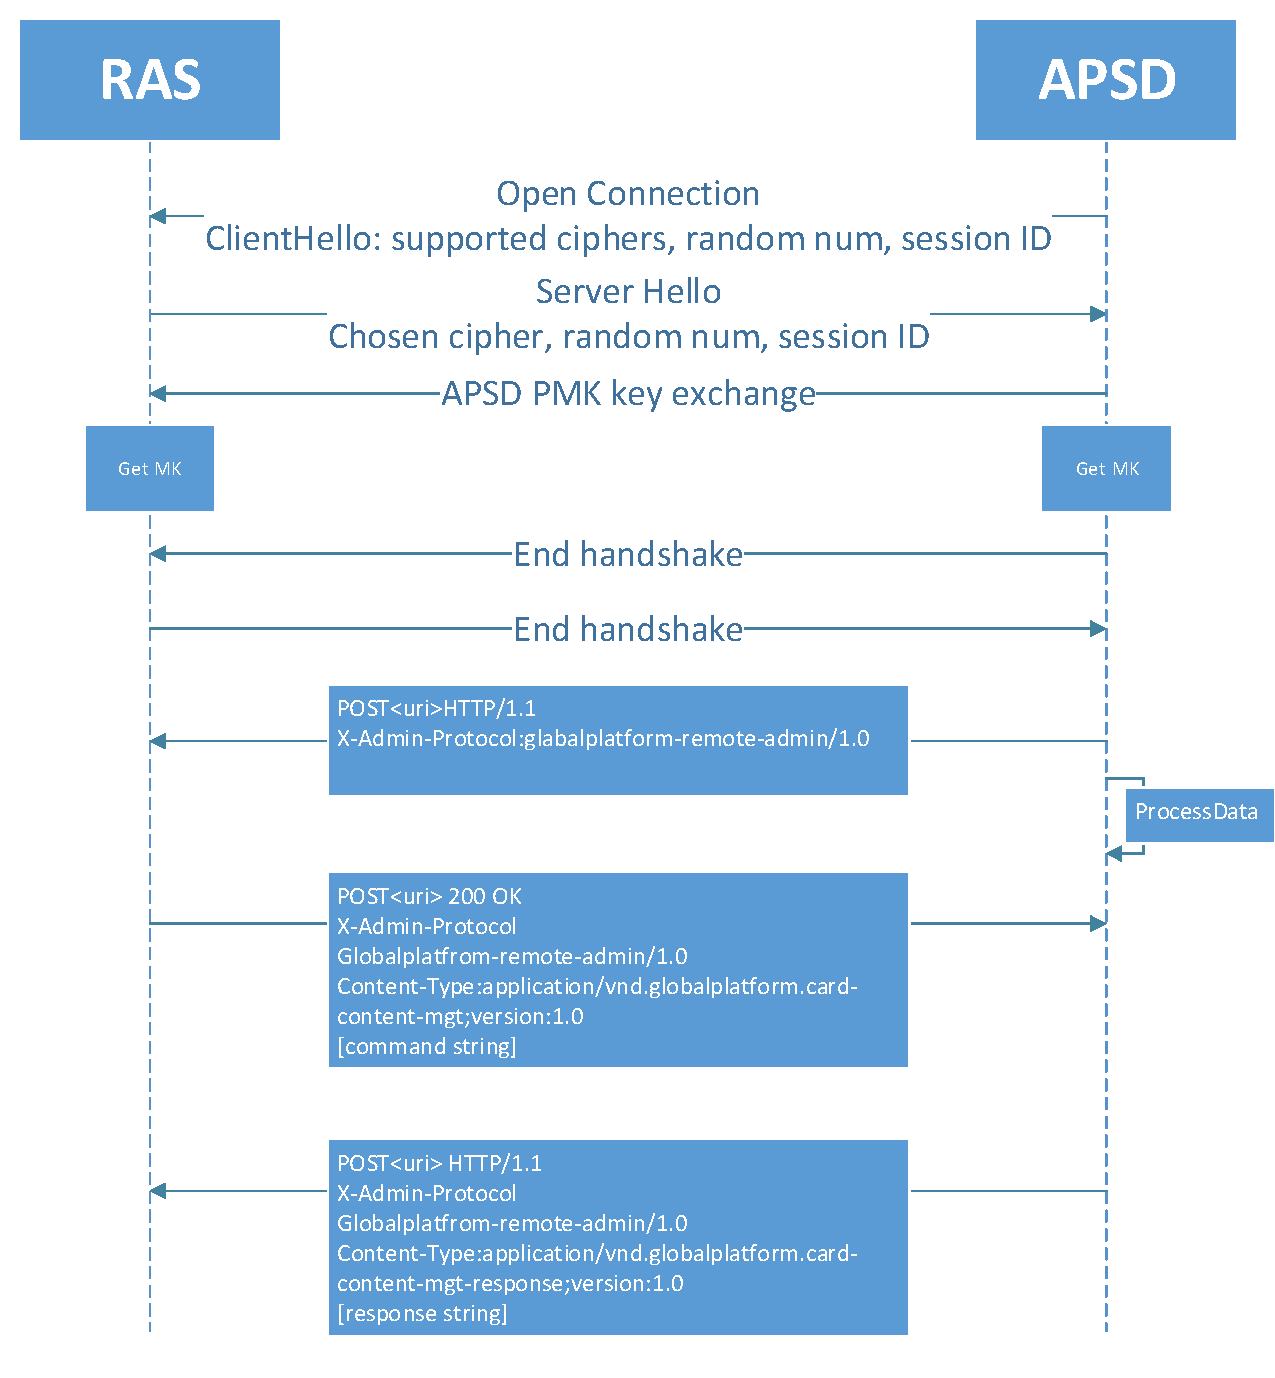
\includegraphics[width=1.2\textwidth]{communication-flow}
		\caption{Class Diagram}
	\label{fig:communication-flow}
\end{figure}

\subsubsection{HTTP Header Format}
The HTTP message sent from remote sever to targeted applet uses following schema\cite{gp}:
\begin{verbatim}
HTTP/1.1 200 OK [or HTTP/1.1 204 No Content CRLF]
X-Admin-Protocol: globalplatform-remote-admin/1.0 CRLF
[X-Admin-Next-URI:  <next-URI> CRLF]
[Content-Type: application/vnd.globalplatform.card-content-mgt
-response;version=1.0 CRLF]
[X-Admin-Targeted-Application: <security-domain-AID> CRLF]
[Content-Length: xxxx CRLF] or [Transfer-Encoding: chunked CRLF]
CRLF
[body]
\end{verbatim}
In the field \emph{security-domain-AID} could be filled the AID of targeted applet.


The HTTP response message sent from applet to remote server uses following schema\cite{gp}:
\begin{verbatim}
POST<URI>HTTP/1.1 CRLF
Host: <Administration Host> CRLF
X-Admin-Protocol: globalplatform-remote-admin/1.0 CRLF
X-Admin-From: <Agent ID> CRLF
[Content-Type: application/vnd.globalplatform.card-content-mgt
-response;version=1.0 CRLF]
[Content-Length: xxxx CRLF] or [Transfer-Encoding: chunked CRLF]
[X-Admin-Script-Status: <script-status> CRLF]
[X-Admin-Resume: true]
CRLF
[body]
\end{verbatim}

The filed \emph{X-Admin-Script-Status} could contain following values:
 \begin{itemize}
  \item \emph{ok}, which means that the previous message is successfully received by applet.
  \item \emph{unknown-application}, which stands for the error, that the targeted applet for previous message can not be found.
\item \emph{not-a-security-domain}, this errors occurs when targeted applet is not a Security Domain.
\item \emph{security-error}, as its name indicates, this values is returned if the security of previous message  can not be checked.
\end{itemize}

\subsubsection{Close Communication Session}
Whenever the communication channel is about to be closed, either because of session security issue, or due to successful finish of communication, remote server will send target applet HTTP message:
 \begin{itemize}
  \item No \emph{X-Admin-Next-URI} field is present in this HTTP message and message body is empty, which will be recognized as final message from remote server and then the session will be closed.
  \item No \emph{X-Admin-Next-URI} filed is present but in this HTTP message body is not empty. The receiver will process the data in body and close the communication session appropriately. But no response message will be generated.
\end{itemize}

\subsection {Commands: Interface between Applet and CAD}
Before concrete implementation of Javacard applet code, the interface, which in essence is a set of commond APDUs and corresponding response APDUs, between applet and CAD must be well defined.  The CommunicationStack support two categories commond APDU:
 \begin{itemize}
  \item The \emph{SELECT} Command APDU, which is used by JCRE to select CommunicationStack applet.
  \item Other command APDUs, which are introduced in order to provide functionalists such as: trigger communication session, process input APDU and etc. To be more specifically:
\begin{itemize}
  \item PIN operation related APDU set
  \item Communication session management APDU set
  \item Data process APDU set
\end{itemize}
\end{itemize}

\subsubsection{SELECT APDU}
The header of this command APDU is fixed and \emph{Lc} indicates the length of CommunicationStack AID. In \emph{Data filed} real AID is saved.
\begin{table}[!htbp]
\caption{SELECT command APDU}
\scalebox{1.3}{%
\begin{tabular}{|l|l|l|l|l|l|l|}
\hline
CLA  & INS  & P1   & P2   & Lc   & Data field                                                                                          & Le  \\ \hline
0x00 & 0xA4 & 0x04 & 0x00 & Length of AID& AID & N/A \\ \hline
\end{tabular}
}
\label{select-apdu}
\end{table}
Two categories of response APDUs are expected, one represents successful processing of \emph{SELECT} command APDU and the other stands for failure.
\begin{table}[!htbp]
\caption{SELECT response APDU}
\label{select-response-apdu}
\scalebox{1.1}{%
\begin{tabular}{|l|l|l|}
\hline
Optional data & Status word & Description                                \\ \hline
No data       & 0x9000      & Successful processing                      \\ \hline
              & 0x6999      & Failed to select CommunicationStack applet \\ \hline               
\end{tabular}
}
\end{table}

\subsubsection{Verify PIN operation}
This APDU command and response set is used to let CommunicationStack applet verify identity of terminal user. Moreover the PIN size is set from four to eight and the verify PIN operation try limit is set to three times.

\begin{table}[!htbp]
\caption{Verify PIN command }
\scalebox{1.2}{%
\begin{tabular}{|l|l|l|l|l|l|l|}
\hline
CLA  & INS  & P1   & P2   & Lc   & Data field    & Le  \\ \hline
0xA0 & 0x11 & 0x00 & 0x00 & length of Data field & PIN & N/A \\ \hline
\end{tabular}
}
\label{verify-command-apdu}
\end{table}

Three categories of response APDUs are expected.

\begin{table}[!htbp]
\caption{Verify PIN response APDU}
\label{verify-response-apdu}
\scalebox{1.2}{%
\begin{tabular}{|l|l|l|}
\hline
Optional data & Status word & Description                                \\ \hline
No data       & 0x9000      & Successful processing                      \\ \hline
              & 0x63C0      & Verification failed \\ \hline      
              & 0x6983      & After 3 times wrong input, pin is block \\ \hline              
\end{tabular}
}
\end{table}

\subsubsection{Reset PIN operation}
This APDU command and response set is introduced to offer end user change PIN service.

\begin{table}[!htbp]
\caption{Reset PIN command }
\scalebox{1.2}{%
\begin{tabular}{|l|l|l|l|l|l|l|}
\hline
CLA  & INS  & P1   & P2   & Lc   & Data field    & Le  \\ \hline
0xA0 & 0x12 & 0x00 & 0x00 & length of Data field &New PIN & N/A \\ \hline
\end{tabular}
}
\label{reset-pin-command-apdu}
\end{table}

Three categories of response APDUs are expected.
\begin{table}[!htbp]
\caption{Reset PIN response APDU}
\label{reset-pin-response-apdu}
\scalebox{1.2}{%
\begin{tabular}{|l|l|l|}
\hline
Optional data & Status word & Description                                \\ \hline
No data       & 0x9000      & Successful processing                      \\ \hline
              & 0x6301      & Verification is required first\\ \hline      
              & 0x6984      & Length of input PIN is wrong \\ \hline              
\end{tabular}
}
\end{table}


\subsubsection{Communication Session Creation}
This APDU command and response set is used to let  CommunicationStack applet initiate the request to establish communication channel and create communication  session above  it. Following commands are supported.

\begin{table}[!htbp]
\caption{Communication session creation command APDUs}
\scalebox{0.95}{%
\begin{tabular}{|l|l|l|l|l|l|l|l|}
\hline
CLA  & INS  & P1   & P2   & Lc   & Data field  & Le  & Description \\ \hline
0xA0 & 0x01 & 0x00 & 0x00 & data filed length & Session parameter& N/A  & create session parameters\\ \hline
0xA0 & 0x02 & 0x00 & 0x00 & data filed length & Session parameter& N/A  & set session parameters\\ \hline
0xA0 & 0x03 & 0x00 & 0x00 &  N/A & N/A& N/A  & create communication session\\ \hline
0xA0 & 0x04 & 0x00 & 0x00 &  N/A & N/A& length of session state & get session state\\ \hline
\end{tabular}
}
\label{trigger-session-apdu}
\end{table}

Following return codes are expected in response APDU:

.\begin{table}[!htbp]
\caption{Trigger Session Return Code}
\label{trigger-session-response-apdu}
\scalebox{1.2}{%
\begin{tabular}{|l|l|l|}
\hline
 Status word & Description                                \\ \hline
 0x9000      & Successful processing                      \\ \hline
 0x66AB      & Array Index out of bounds exception \\ \hline           
 0x665E      & Security exception \\ \hline 
 0x6600      & Nullpointer  exception \\ \hline  
 0x6C00      & UnKnown  exception \\ \hline      
\end{tabular}
}
\end{table}


\subsubsection{Close Communication Session }
This APDU command and response set is used to correctly close  communication channel.


\begin{table}[!htbp]
\caption{Close Session command APDU}
\scalebox{1.3}{%
\begin{tabular}{|l|l|l|l|l|l|l|}
\hline
CLA  & INS  & P1   & P2   & Lc   & Data field                                                                                          & Le  \\ \hline
0xA0 & 0x50 & 0x00 & 0x00 & 0x00 & N/A& N/A \\ \hline
\end{tabular}
}
\label{close-session-apdu}
\end{table}

Following return codes are expected in response APDU:

.\begin{table}[!htbp]
\caption{Close Session Return Code}
\label{close-session-response-apdu}
\scalebox{1.2}{%
\begin{tabular}{|l|l|l|}
\hline
 Status word & Description                                \\ \hline
 0x9000      & Successful processing                      \\ \hline
 0x6032      & Failed to close session \\ \hline             
\end{tabular}
}
\end{table}

\subsubsection{Process Communication Data }
This APDU command and response set is used to provide functionalities to perform command processing between cellphone and  other smart home device. 


\begin{table}[!htbp]
\caption{Process data command APDUs}
\scalebox{0.98}{%
\begin{tabular}{|l|l|l|l|l|l|l|l|}
\hline
CLA  & INS  & P1   & P2   & Lc   & Data field  & Le \\ \hline
0xA0 & 0x20 & 0x00 & 0x00 & data filed length & desired target's public key & PK length \\ \hline
0xA0 & 0x21 & 0x00 & 0x00 & data filed length & command data & response length \\ \hline
\end{tabular}
}
\label{process-data-cmd-apdu}
\end{table}

Following return codes are expected in response APDU:

.\begin{table}[!htbp]
\caption{Process data Return Code}
\label{process-data-res-apdu}
\scalebox{1.2}{%
\begin{tabular}{|l|l|l|}
\hline
 Status word & Description                                \\ \hline
 0x9000      & Successful processing                      \\ \hline
 0x6A80      & error in data filed \\ \hline        
 0x6A81      & required device not found \\ \hline        
 0x6A82      & required service not found \\ \hline   
 0x6A83      & required record not found \\ \hline                
\end{tabular}
}
\end{table}